\documentclass[12pt]{article}
\title{Macromolecular Docking - project seminar}
\author{Peter M\"uhlbacher - a1253030}

\usepackage{amsmath, amsthm, amsfonts}
\usepackage{hyperref}
\usepackage{todonotes}
\usepackage{natbib}
\usepackage{rotating}
\usepackage{mathrsfs}
\usepackage[]{algorithm2e}

\theoremstyle{definition}\newtheorem*{definition}{Definition}
\newtheorem*{theorem}{Theorem}
\newtheorem*{lemma}{Lemma}
\newtheorem*{proposition}{Proposition}
\newtheorem*{corollary}{Corollary}
\theoremstyle{definition}\newtheorem*{remark}{Remark}

\begin{document}
\maketitle

\begin{abstract}
This paper deals with the application of mathematical methods for macromolecular docking. The goal is to write a program to determine the likeliness of a configuration of two proteins. Thus the first section is based on elaborating on the theoretical background and introducing notation used in chemistry literature. The second section deals with translating qualitative requirements into quantitative statements by introducing and analyzing the Lennard-Jones potential. The third and fourth sections deal with encountered mathematical difficulties when calculating the potential. The sixth section describes the implementation and the last section reviews the results.
\end{abstract}

\section{Terminology}
Throughout the paper some chemistry terminology will be used. The most important terms will be introduced in this section.
Furthermore elements from $\mathbb R^3$ will be indicated by a bold typeface.

\subsection{Fundamentals on Proteins}
This subsection will refer a lot to \cite{burger}.

\subsubsection{Polypeptide chains}
An amino acid\footnote{Note the ``exception'' proline.} is a molecule which contains an amino $-NH_2$ and a carboxyl $-COOH$ functional group.

\begin{figure}
\caption{Illustration of an amino acid. \cite{Neumaier97}}
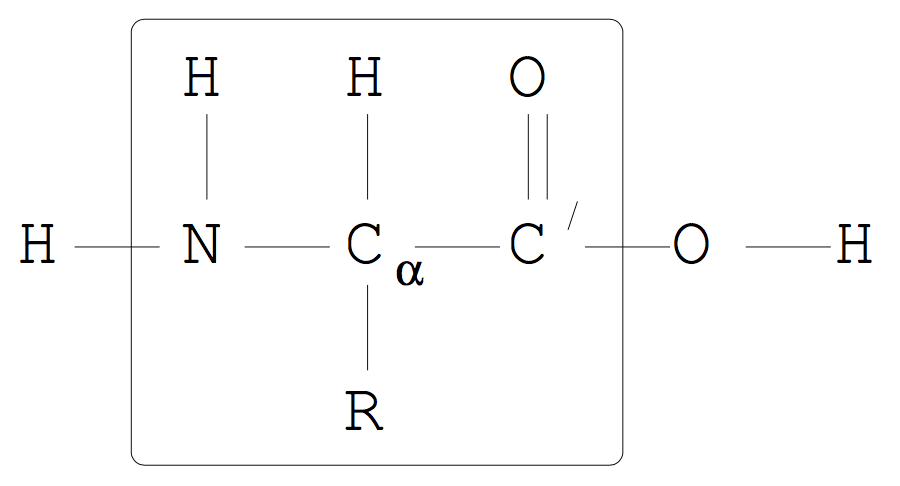
\includegraphics[width=0.7\linewidth]{aminoacid.png}
\end{figure}


Nineteen of the twenty amino acids in proteins are $\alpha$-amino acids, which have the form $H_2N - C_\alpha H - COOH$, where $R$ determines each amino acid.

A peptide bond forms between the carboxy terminal $-CO$ of one amino acid and the amino terminal $-NH$ of a neighbouring amino acid by the removal of a water molecule.

Peptides longer than around 80 amino acids are called polypeptides, and peptides with biological function are called proteins. Proteins usually have less than 2000 amino acids, but there are proteins with around 5000 amino acids.
\\~\\
A protein's $-N-C_\alpha-C-$ chain is commonly referred to as the protein's backbone.

When two or more amino acids combine to form a peptide, two $H$ and one $O$ are removed---what remains of each amino acid is called a \textit{residue}.

\subsection{Structures}
\subsubsection{Primary structure}\label{subsubsec:primary_structure}
A protein's primary structure is its amino acid chain $(A_i)_i$ where $\{A_k\}_{k\in\{1,\dots,20\}}$ is the set of amino acids. Note that this is a linear structure without closed paths or bifurcations.

\subsubsection{Secondary structure}
The secondary structure refers to a protein's spatial arrangement of amino acid residues which are ``nearby'' in the sequence. Examples might be $\alpha$-helices or $\beta$-sheets.\footnote{However, this is just mentioned for completeness' sake and will not be used (and thus not be explained) in this paper.}

\subsubsection{Tertiary structure}
The tertiary structure is the protein's three-dimensional structure, as defined by the single atoms' coordinates in $\mathbb R^3$. This representation is particular interesting as it determines the protein's function.

\subsubsection{Quaternary structure}
There are multiple definitions for the quaternary structure. In this paper the following definition from \cite{berg} is used, which characterizes it as the ``spatial arrangement of multiple folded proteins and the nature of their interactions''.


\subsection{Coordinates}\label{subsec:coords}
As will be discussed later, a big part of problems like protein folding/docking is converting between different kinds of coordinate systems. Those will be defined in this subsection.

\subsubsection{Bond vector}
Assigning to each atom $i$ a position $\bold x_i$ in a Cartesian coordinate system, one can define the \textit{bond vector} $p$ of a pair of atoms $(i,j)$ to be $\bold x_j - \bold x_i$.

The \textit{bond length} of $\{i,j\}$ is then defined as the norm $\|p\|$ of their bond vector.

\subsubsection{Bond angles}
Given a triple of atoms $(i,j,k)$ and their bond vectors $p,q$ (for the pairs $(i,j)$ and $(j,k)$ respectively) their \textit{bond angle} $\varphi\in[0,\pi)$ is defined by:

$$cos\varphi = \frac{\langle p,q\rangle}{\|p\|\|q\|}, \,sin\varphi = \frac{\|p\times q\|}{\|p\|\|q\|}$$

\subsubsection{Dihedral angles}
Given a quadruple of atoms $(i,j,k,l)$ and their bond vectors $p,q,r$ (for the pairs $(i,j)$, $(j,k)$ and $(k,l)$ respectively) their \textit{dihedral angle} $\theta\in[-\pi,\pi)$ is defined by:

$$cos\theta = \frac{\langle p\times q,q\times r\rangle}{\|p\times q\|\|q\times r\|}, \,sin\theta = \frac{\langle r\times p,q\rangle\|q\|}{\|p\times q\|\|q\times r\|}$$ 

\begin{remark}[Notation]
In chemistry literature the bond angles are usually denoted by the letter $\theta$, and the dihedral angles describing the torsion around the backbone $N-C_\alpha, C_\alpha-C$, and $C-N$ bonds by the letters $\varphi,\psi,\omega$, respectively; dihedral angles in the side chain by $\chi$.

This work, however, focuses more on the mathematical part, not distinguishing between the various types of dihedral angles and denotes bond and dihedral angles, as in their definitions, by $\varphi$ and $\theta$ respectively.
\end{remark}


\subsubsection{Internal coordinates}\label{subsubsec:int_coords}
Throughout this paper, unless otherwise mentioned, \textit{internal coordinates} will refer to the set of bond lengths, bond angles, dihedral angles\footnote{Those values completely determine a protein's tertiary structure.} and a point of reference in $\mathbb R^3$.

Usually only a certain subset of dihedral angles, e.g. only the backbone's, is allowed to vary.

This representation is particularly useful for altering a molecule in a chemically meaningful way. For example, rotating some bonds is much more likely, i.e. does not cause a big difference in the potential function, than just arbitrarily changing Cartesian coordinates of the single atoms.

The internal coordinates of a single atom $i$ are defined as $(l_i,\varphi_i,\theta_i)$, where $l_i$ is the bond length to $i$'s parent $j$, $\varphi_i$ is the bond angle of the triple $(i,j,k)$, where $k$ is $j$'s parent, and $\theta_i$ is the dihedral angle of the quadruple $(i,j,k,l)$, where $l$ is the $k$'s parent.

\subsubsection{Absolute coordinates}\label{subsubsec:abs_coords}
\textit{Absolute coordinates} will refer to the set of Cartesian coordinates of every single atom in a molecule. This yields a $3N$-dimensional state space for a protein with $N$ atoms.

This representation is particularly useful for calculating potentials which are usually written in terms of mutual distances. Those distances are (except for pairs of atoms that are bonded) hard to calculate from internal coordinates.

\subsection{Docking}\label{subsec:docking_def}
The problem of finding metastable states (local minima of the potential) and/or the ground state (the minimum of the potential) of a system of two proteins interacting with each other is called \textit{protein docking}.

Usually the internal coordinates of one of the two proteins (the ``receptor'') is held fixed, while a subset of internal coordinates can vary for the other one (the ``ligand'').

The special case where this subset is empty (i.e. the internal coordinates of both proteins are fixed and only global translations/rotations are admissible) is called \textit{fixed docking}, while the more general case is called \textit{flexible docking}.



\section{Lennard-Jones Potential}
The Lennard-Jones potential, or ``12-6 potential'', is a model to approximate the pairwise interaction of neutral particles. In this paper it is denoted by $LJ_{M_i,M_j}$ and is set to

$$LJ_{M_i,M_j}(r) = \frac{A_{M_i,M_j}}{r^{12}}-\frac{B_{M_i,M_j}}{r^6}.$$

\begin{remark}[Notation]
	In the literature there are a number of different ways of expressing the Lennard-Jones potential. One of the most popular ones will be addressed in  subsection \ref{subsec:LJ_interpretation}.
\end{remark}

\subsection{Physical Interpretation}\label{subsec:LJ_interpretation}
The indices $M_i$ and $M_j$ determine the potential's parameters $A$ and $B$. The argument $r$ is the distance between two particles. One can think of $M_i$ and $M_j$ as the atom types that interact differently---this accounts for two carbon atoms (potentially) having a different equilibrium distances and behaviour under perturbations as a carbon and an oxygen atom.

\begin{figure}
\caption{Plot of the Lennard-Jones potential with fitted parameters for a pair of carbon atoms.}
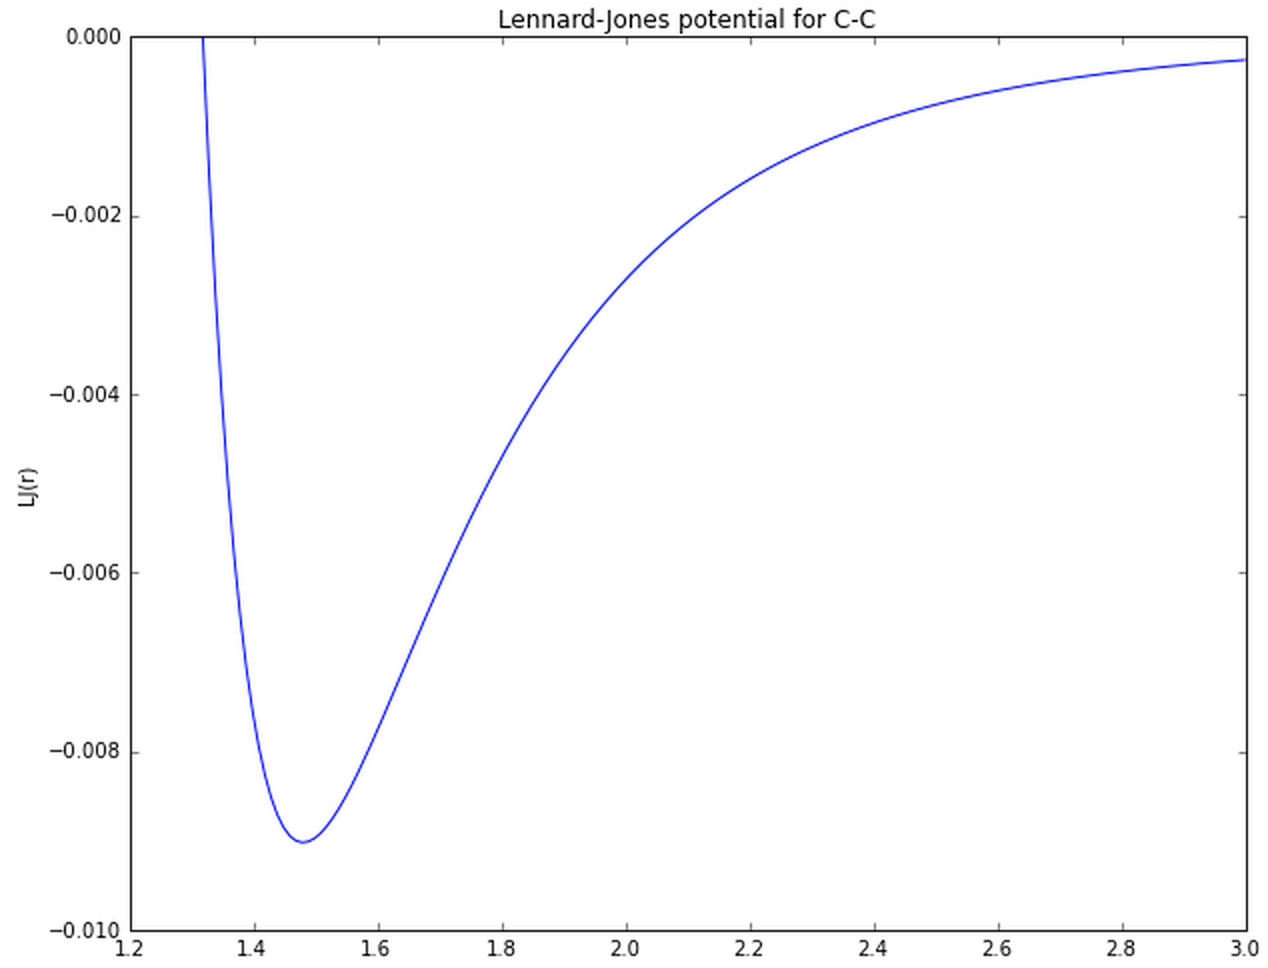
\includegraphics[width=1\linewidth]{LJ.png}
\end{figure}

As there are only finitely many atom types and because of symmetry considerations one can interpret $A$ and $B$ as symmetric ``parameter matrices''. Interpreting $A_{M_i,M_j}$ as the strength of the Pauli-repulsion and $B_{M_i,M_j}$ as the attractive long-range term we can also restrict $A$ and $B$ to matrices with real entries strictly greater than zero.

Another common definition of the Lennard-Jones potential is $\varepsilon\left[\left(\frac{r_m}{r}^{12}\right)-2\left(\frac{r_m}{r}^6\right) \right]$, which relates to the above definition as follows\footnote{The indices ${M_i,M_j}$ have been omitted for readability.}:

\begin{itemize}
	\item $\varepsilon = \underset{r}{\operatorname{min}}\,LJ(r) = \frac{B^2}{4A}$ is the depth of the potential well and thus (i.a.) characterizes how the system behaves under perturbations.
	\item $r_m = \underset{r}{\operatorname{argmin}}\,LJ(r) = \sqrt[6]{2\frac{A}{B}}$ determines the equilibrium distance of the two atoms of types $M_i$ and $M_j$.
\end{itemize}

\subsection{Feasibility}
One has to keep in mind that this model is not ``reality''. It is an empirical approximation in the sense that it has to be fitted to data to yield optimal results. Thus the above interpretations are nice to gain some intuition, but they should not be taken literally. 

For example, distinguishing between $C$ and $C_\alpha$, even though they clearly are the same type of atom, will yield better results as this provides us with more degrees of freedom and may, to some extent, account for other properties that are not included in the model being used. Examples for such properties (in this case where the potential is modelled as a sum of Lennard-Jones potentials over all pairs of atoms of a protein\footnote{For the concrete implementation of the potential for this paper see subsection \ref{subsec:LJ_implementation}.}) include dipole-dipole interactions which lead to secondary structures like the $\alpha$-helix and thus cannot be omitted without losing a lot of predictive power.

These considerations should motivate the following digression on parameter estimation.


\subsection{Parameter Estimation}\label{subsec:LJ_paramestimation}
Let $M$ be some molecule (in our case a protein), $X_M$ its internal coordinates, $A,B$ the parameter matrices as described in subsection \ref{subsec:LJ_interpretation} and $U_{A,B}$ the potential as defined in subsection \ref{subsec:LJ_implementation} as a function of the molecule's internal coordinates $X$.

\subsubsection{Casting it as an optimization problem}

Observing that ``$M$ is in a metastable state'' is equivalent to $$\nabla U_{A,B}(X_M)=0,$$
it is natural to choose $A,B \in (\mathbb R^+)^{n\times n}$ (where $n$ is the number of different substances one wants to differentiate between) as

\begin{equation}\label{eq:param_estimation}
	(A,B)=\underset{(A,B)}{\operatorname{argmin}} \sum_{M^i\in\text{training set}}\|\nabla_X U_{A,B}(X_{M^i})\|.
\end{equation}

However, this is a homogenous system, so approaching this optimization problem naively one would only get the trivial solution where all matrix entries converge towards zero. Hence we fix $A_{11} = \textit{const} > 0$ and express all other parameters in terms of $A_{11}$, i.e.: $\tilde A_{ij} = A_{11}A_{ij}$ and $\tilde B_{ij} = A_{11}B_{ij}$.

\subsubsection{Making an initial guess}

For many optimization algorithms choosing a good starting point, even more so in high dimensions, is crucial for their success.

To calculate an initial ``guess'' one option is to project the true optimization problem \eqref{eq:param_estimation}, which is in $n(n+1)-1$ dimensions, for $n$ denoting the number of different atom types one wants to be able to differentiate.

One crude, but kind of canonical way of doing that is to assume that the Lennard-Jones potential simply does not depend on the type of atom, i.e. setting $A_{ij}$ and $B_{ij}$ to $A_{11}$ and $B_{11}$ for $(i,j)\in \{1,\dots,n\}\times\{1,\dots,n\}\setminus (1,1)$, respectively. In this case, where $A_{11}$ is a fixed constant this reduces to a one dimensional optimization problem.

For the experimental results see figure \ref{fig:param_estimation_projection}.

\begin{figure}
\caption{Projection of the optimization problem in $n(n+1)-1$ dimensions onto a $1$-dimensional subspace ($B_{11}$ is the only non-constant parameter, $A_{ij}=1, B_{ij}=B_{11}$)}
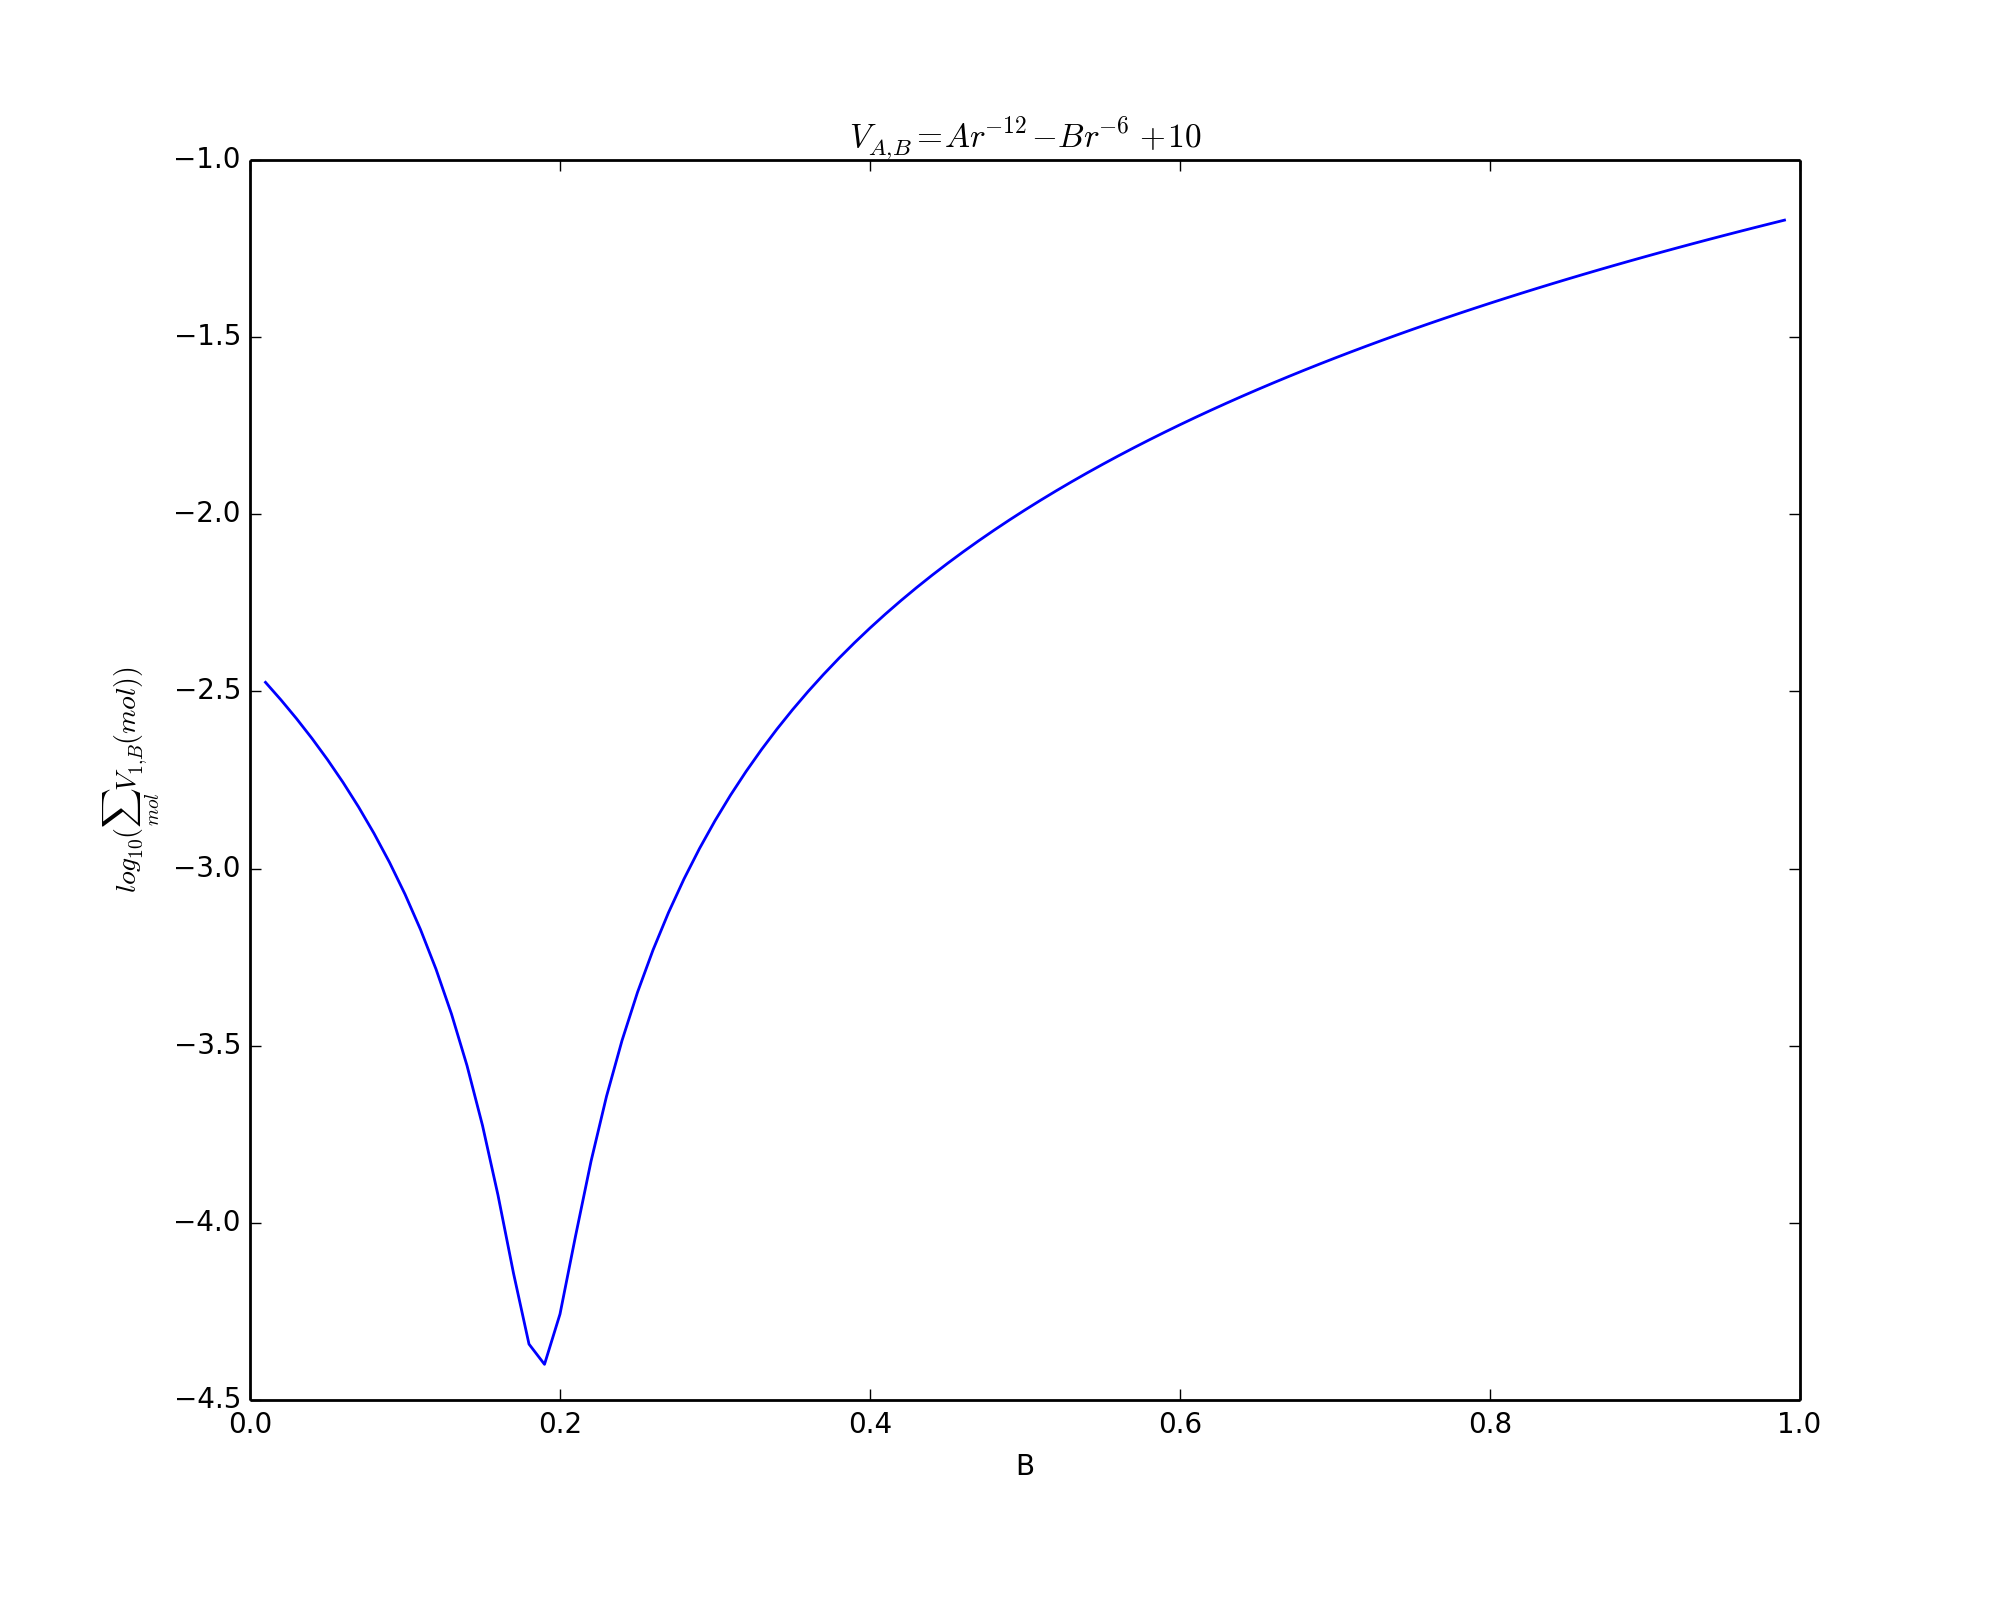
\includegraphics[width=1\linewidth]{sumoverU.png}
\label{fig:param_estimation_projection}
\end{figure}




\section{Coordinate Conversion}
As already mentioned in subsections \ref{subsubsec:int_coords} and \ref{subsubsec:abs_coords} one of the most important parts of working with proteins (including protein folding and in particular protein docking) is the conversion between internal and absolute coordinates for chemically meaningful changes to the molecule and calculating its potential, respectively.

Given some point of reference, the distances, bond and dihedral angles it does not seem to be a big challenge to apply some trigonometry to calculate one atom's position after another depending on the previous atoms' positions, however, that is just the problem: Traversing a protein's chain-like structure naively as described above will result in an accumulation of rounding errors that makes this conversion useless for calculating the potential.

Another issue is the time needed for those conversions. One would like to write the potential as a function of internal coordinates, so that the gradient indicates which (chemically meaningful) changes would have to be made\footnote{The difference between using internal and absolute coordinates for calculating the potential is a little bit like the difference between using a Lagrangian or a Hamiltonian to describe the evolution of a system.}, but then one has to calculate the absolute coordinates from the internal coordinates for every single evaluation of the potential.

\begin{remark}[Conversion from absolute to internal coordinates]
	The conversion from absolute to internal coordinates has already been described in subsection \ref{subsec:coords}. It is not so prone to accumulation of rounding errors and faster.
\end{remark}

\subsection{Calculating the Children's Absolute Coordinates}
As already suggested above, and as motivated by the tree-like structure of a protein, one can formulate the problem of converting the internal coordinates to absolute coordinates as finding a recursive function that calculates for each atom its ``children''.
For this task the \textit{natural extension reference frame} algorithm (short: NeRF), as introduced by \cite{nerf} has been implemented.

\subsubsection{NeRF}\label{subsubsec:nerf}
This function, depending on the atom's internal and its three ancestors' absolute coordinates, will henceforth be referred to as \texttt{nerf()}.

First of all we define a recursive function \texttt{buildChildren()}:

\begin{algorithm}[H]
	\KwData{\texttt{parent}(Node), \texttt{A}(double[]), \texttt{B}(double[])}
	\KwResult{calculated coordinates are added to the \texttt{molecule} list}
 
 	\texttt{C} $\leftarrow$ \texttt{parent.coord}\;
	\For{\texttt{child} in \texttt{parent.children}}{
		\texttt{child.coord} $\leftarrow$ \texttt{nerf(A,B,C,child.dist,child.theta,child.phi)}\;
		\texttt{molecule.append(child.coord)}\;
		\texttt{buildChildren(child,B,C)}\;
	}
	\caption{buildChildren()}
\end{algorithm}

Note that in the actual implementation the NeRF algorithm is called with the additional (redundant, in the sense that it could be computed from the other parameters) parameter \texttt{parent.dist} to save one additional computation.

Also, the first three levels' atoms are assumed to be static due to the internal coordinates' nature (they do not have a well-defined dihedral angle). In practice these first three levels would be the first residue's $N$, $CA$, $CB$ (in case there is one) and $C$.
To bypass this problem, one could have defined ``imaginary'' auxiliary atoms at some coordinates, fixed by convention, in order to retrieve the missing internal coordinates for the first residue's $CA$, etc., but this has not been done as it would have complicated the implementation without any apparent improvements.

The NeRF algorithm is implemented as follows:

\begin{algorithm}[H]
	\KwData{$A$(double[]), $B$(double[]), $C$(double[]), $R$(double), $\varphi$(double), $\theta$(double), $lbc$(double), $D$(double[])}
	\KwResult{absolute coordinates of the child node}
 	
 	\If{\texttt{D} is not passed as argument}{
 		$\text{sinphi} \leftarrow sin\varphi$\\
 		$D\leftarrow R(cos\varphi,\text{sinphi}\,cos\theta,\text{sinphi}\,sin\theta)^\dagger$
 	}
 	$AB \leftarrow B-A$\\
 	$BC \leftarrow C-B$\\
 	$bc \leftarrow \frac{BC}{lbc}$\\
 	$N  \leftarrow AB\times bc$\\
 	$n  \leftarrow \frac{N}{\|N\|}$\\
 	$M  \leftarrow (bc,n\times bc,n)$\\
 	
 	\Return $\langle M,D\rangle+C$
 	
	\caption{nerf()}
\end{algorithm}

According to \cite{nerf} NeRF is not only faster, but also more stable from a numerical point of view.
Furthermore it provides a natural way of reusing interim results for occasions when a parent node's internal coordinates changed, but the node's internal coordinates stayed the same, which translates to $D$ staying the same.

Alternatives include naive methods as suggested above, quaternions and different ways of combining rotation matrices in three or four dimensions. Latter also includes translations in three dimensions by introducing another dimension.





\section{Computation of the Gradient}
Computing the gradient is interesting for multiple reasons:
\begin{enumerate}
	\item Optimization algorithms like gradient descent make heavy use of gradients. As pointed out in subsection \ref{subsec:docking_def} the docking problem is essentially an optimization problem where one wants to minimize some potential for a system of two proteins.
	\item As elaborated on in subsection \ref{subsec:LJ_paramestimation} the gradient is important to optimize for the parameters of the Lennard-Jones potential.
	\item Considering a single protein, the potential is invariant under global translations and rotations, so the only non-zero terms in the gradient are the ones for its dihedral angles\footnote{Bond lengths and bond angles are fixed.} $\{\frac{dU}{d\theta_i}\}_i$. When one wants to find a subset of parameters (i.e. of internal coordinates) which are kept variable, the magnitude of their entry in the gradient $|\frac{dU}{d\theta_i}|$ is a suitable measure as small changes in those variables with bigger magnitude have a bigger effect on the potential.
\end{enumerate}

The computation of the gradient of a function depending on thousands of variables---for (almost) every atom there is a dihedral angle---cannot be done by resorting to difference quotients and trying to take their limits. This is not only due to their inaccuracy, but also due to the computational complexity of having to evaluate the potential at least two times for every entry in the gradient.

Symbolic differentiation is also not favourable since it is not only very complex and hard to hard to maintain in practice, but also tends to produce complicated expressions resulting in an accumulation of rounding errors.

To deal with this problem automatic differentiation was introduced.

\subsection{Automatic Differentiation}
The basic idea is to write every expression $z$ as a composition of simpler functions $z=f(y), y=g(x)$, then applying the chain rule to write $\frac{dz}{dx}$ as $\frac{dz}{dy}\frac{dy}{dx}$ and calculating $\frac{dz}{dy}$, $\frac{dy}{dx}$ separately.

Two extreme cases of traversing the chain rule are
\begin{enumerate}
	\item Forward accumulation: Traversing from the inside to the outside, i.e. first evaluating $\frac{dy}{dx}$ and then $\frac{dz}{dy}$.
	\item Reverse accumulation: Traversing from the outside to the inside, i.e. first evaluating $\frac{dz}{dy}$ and then $\frac{dy}{dx}$.
\end{enumerate}

While the case where $f\circ g : \mathbb R \rightarrow \mathbb R$ looks trivial, the multivariate case $y = F(x), F:\mathbb R^n \rightarrow \mathbb R^m$ is a little bit more work and will be dealt with here in a more general framework than above.\footnote{The following will rely heavily on \cite{Neumaier01}, p.305ff.}

To do so it is convenient to introduce the following vectors/matrices:

\begin{itemize}
	\item The auxiliary vector $z\in\mathbb R^l$ storing the interim results from the calculation of $F(x)$ such that each $z_i$ can be computed with a single operation from one or two $z_j$ (where $j<i$) or $x_j$.
	\item The projection $P\in\{0,1\}^{m\times l}$, with exactly one 1 in each row, such that $y=Pz$.
\end{itemize}

Using those definitions one can write 

\begin{equation}\label{eq:autodiff_z_as_H}
	z=H(x,z),
\end{equation}

 where $H(x,z)_i = z_i$. Thus the partial derivatives $H_x$ and $H_z$ (which is lower triangular) are extremely sparse.

Differentiating \eqref{eq:autodiff_z_as_H} gives

\begin{equation}\label{eq:autodiff_dzdx}
	\frac{\partial z}{\partial x} = H_x(x,z)+H_z(x,z)\frac{\partial z}{\partial x},
\end{equation}

which yields:

$$\frac{\partial z}{\partial x} = (I-H_z(x,z))^{-1}H_x(x,z).$$

\subsubsection{Forward automatic differentiation}

Now one writes $F'(x) = \partial y/\partial x = P\partial z/\partial x$ to get $$F'(x) = P{\underbrace{(I-H_z(x,z))}_{\text{lower triangular}}}^{-1}H_x(x,z)$$

and solves \eqref{eq:autodiff_dzdx} by using forward substitution on 

\begin{equation}\label{eq:autodiff_forward}
	(I-H_z)\frac{\partial z}{\partial x} = H_x.
\end{equation}

This process is called \textit{forward automatic differentiation}.

\subsubsection{Backward automatic differentiation}
Consider the adjoint problem by writing

$$F'(x)^\dagger = H_x(x,z)^\dagger\underbrace{(I-H_z(x,yz))^{-\dagger}P^\dagger}_{=:K}.$$

$K$ can be found by using back substitution on 

\begin{equation}\label{eq:autodiff_backward}
	{\underbrace{(I-H_z)}_{\text{upper triangular}}}^\dagger K=P^\dagger.
\end{equation}

This way of obtaining $$F'(x) = K^\dagger H_x(x,z)$$ is called \textit{reverse} or \textit{backward automatic differentiation}.

\subsubsection{Forward or backward automatic differentiation?}
A disadvantage of backward automatic differentiation is that $H_x(x,z)$ has to be stored fully while, for the forward automatic differentiation case, it can be computed on the fly for \eqref{eq:autodiff_forward}.

However, if $m \ll n$, which is the case for potentials (i.e. the special case of $F:\mathbb R^n \rightarrow \mathbb R$), \eqref{eq:autodiff_forward} has $n$ columns on the r.h.s. while \eqref{eq:autodiff_backward} has only $m$ columns. In the above mentioned special case this means that $K$ is nothing more but a scalar.

It can be shown more rigorously that in cases like ours backward automatic differentiation is faster\footnote{Depending on the implementation and hardware.}, but above considerations should provide good heuristic arguments.

\section{Implementation}

\subsection{Data Structure}
While the first implementation used a recursive data structure to store the nodes the latest version resorts to a linear structure where every molecule is represented as a tuple consisting of the following lists:

\begin{itemize}
	\item \texttt{atomnames}: A list of the atoms' atom names as given in PDB files' \texttt{ATOM} entries.
	\item \texttt{X}, \texttt{Y}, \texttt{Z}: Lists storing the atoms' absolute coordinates relative to its reference point.
	\item \texttt{dists}, \texttt{phis}, \texttt{thetas}: Lists storing the single atoms' internal coordinates.
	\item \texttt{children}: The $i$-th entry is a list of integers denoting the indices of the atoms that the $i$-th atom is a parent node of.
	\item \texttt{Ds}: As discussed in subsubsection \ref{subsubsec:nerf} this list stores interim results for the \texttt{nerf} algorithm (for the parameters as given in the fields describing the internal parameters).
\end{itemize}

This representation has been proven to be more accessible than the recursive representation, is faster and does not cause difficulties like exceeding languages' maximal recursion limits for big molecules.

\subsection{Lennard-Jones Potential}\label{subsec:LJ_implementation}
Let $X = (x,y,z,\alpha,\beta,\gamma,\theta_1,\dots,\theta_N)$ be a vector storing free parameters, where $(x,y,z)=:\bold x$ denote the molecule's point of reference (i.e. absolute coordinates of the PDB file's first atom), $\alpha,\beta,\gamma$ specify the global rotation of the molecule as given by the following rotation matrices

$$R_x(\alpha_1) = \left(\begin{array}{ccc}
1 & 0 & 0 \\
0 & \text{cos}\,\alpha & -\text{sin}\,\alpha \\
0 & \text{sin}\,\alpha &  \text{cos}\,\alpha \end{array}\right),$$ $$R_y(\beta)=\left(\begin{array}{ccc}
\text{cos}\,\beta & 0 & -\text{sin}\,\beta \\
0 & 1 & 0\\
\text{sin}\,\beta & 0 &  \text{cos}\,\beta\end{array}\right)$$ and $$R_z(\gamma) = \left(\begin{array}{ccc}
\text{cos}\,\gamma & -\text{sin}\,\gamma & 0 \\
\text{sin}\,\gamma &  \text{cos}\,\gamma & 0 \\
0 & 0 & 1 \end{array}\right)$$

and $\theta_1,\dots,\theta_N$ represent varying dihedral angles.
	
Thus the absolute coordinates of the molecule's $i$-th particle with relative coordinates $\bold a_i$ are given by

$$R_x(\alpha)R_y(\beta)R_z(\gamma)\mathbf a_i + \mathbf x.$$
	
\begin{remark}[Number of dihedral angles]
	The $n$ in $\theta_1,\dots,\theta_N$ does not have to be equal to the numbers of atoms of the molecule, since in most cases one selects only some subset of dihedral angles which are not fixed.
\end{remark}

\begin{remark}[Other internal coordinates]
	Other internal coordinates (bond length and bond angles) are usually (and in particular in this work) being held fixed. The justification is not of mathematical, but rather of chemical nature.
\end{remark}

Now let $M^1(X)=M^1$ be the flexible and $M^2$ the fixed molecule and $\{\bold a^1_i\}_i, \{\bold a^2_j\}_j$ their relative coordinates, respectively, then we can finally write the potential $U(X)$ of the system of two molecules as a function of the vector $X$ determining the structure of the flexible molecule $M^1$ as discussed above:

\begin{equation}\label{eq:potential_of_system}
	U(X) =
\underbrace{\sum_{i=1}^{|M^1|}\sum_{j>i}^{|M^1|}LJ_{M^1_i,M^1_j}(\|\bold a^1_i-\bold a^1_j\|)}_{\text{internal energy of }M^1} + \underbrace{\sum_{i=1}^{|M^1|}\sum_{j=1}^{|M^2|}LJ_{M^1_i,M^2_j}(\|\bold a^1_i-\bold a^2_j\|)}_{\text{interaction of }M^1\text{ and }M^2}
\end{equation}

Note that pairwise interactions of the fixed molecule are omitted since they do not depend on $X$ and for optimization a constant additive factor does not make any difference.

\subsection{Differentiation}
When using software for automatic differentiation one has to take care of recursive functions (e.g. \texttt{buildChildren()}) since they cause recursions for some libraries like AutoGrad\footnote{See \cite{autograd}.} and that may cause maximal recursion errors.

\subsection{PDB}
The PDB file format is a widely used format to store information on proteins. In this section only a tiny subset of its conventions, in particular those that have been used in the implementation, will be introduced. As the PDB file format takes account of the characters' column\footnote{A notorious example is that \texttt{CA\_\_} would stand for calcium, while \texttt{\_CA\_} would stand for the $C_\alpha$ carbon element in a protein's backbone, assuming both entries were in columns 13-16.} in each line underscores are being used in this section to highlight spaces.

Generally there are different kind of \textit{entries}: An entry corresponds to a line in the PDB file and its type is determined by a line's characters in the first six columns.
 
For this project it was sufficient to concentrate on the \texttt{ATOM\_\_} type. In the following table only the fields that were needed will be elaborated on.

\begin{center}
    \begin{tabular}{ | p{1.45cm} | l | l | p{5cm} |}
    \hline
    Columns & Data type & Field & Definition \\ \hline
    1-6 & Character & entry type & In this case this will always be \texttt{ATOM\_\_}. \\ \hline
    7-11 & Integer & serial number & The (PDB file's) $i$-th atom's serial number is $i$. \\ \hline
    13-16 & Character & atom name & The first two characters (which are right aligned, so in case of elements that are denoted by a single letter, like oxygen, it is \texttt{\_O} and \textit{not} \texttt{O\_}!) determine the chemical element, the third character is the remoteness indicator and the fourth character is the branch indicator.\\\hline
    18-20 & Character & residue type & Three character abbreviation for each of the 20 amino acids. \\\hline
    23-26 & Integer & residue number & Counter for the residues. \\\hline
    31-38, 39-46, 47-54 & Floating & X,Y,Z coordinates & Coordinates in Angstrom relative to some point of reference. \\\hline
    \end{tabular}
\end{center}

An example for a carbon atom in threonine, where this carbon atom is the protein's 4387th atom and the threonine the protein's 146th residue would be:
\\~\\
\texttt{ATOM\_\_\_4387\_\_CG1\_THR\_\_\_146\_\_\_\_\_\_29.948\_\_11.544\_\_57.310\_\_\dots}
\\~\\
In the following the terms ``node'' and ``atom'' will be used interchangeably as we are viewing the protein as a graph. 

Still, the \textit{remoteness indicator} and the \textit{branch indicator} have yet to be defined. To do this it is necessary to view a protein as a tree-like graph structure. As already discussed in subsubsection \ref{subsubsec:primary_structure}, considering a protein as a tuple of residues yields a linear, graph representation\footnote{Its vertices are the residues and the edges connect two adjacent residues.} without bifurcations or circles. The same holds true if one considers a graph on the atomic level in terms of its backbone atoms which would result in a subdivision of the above mentioned graph. However, if one considers the graph where the vertices are all the protein's atoms and its edges correspond to their bonds there are bifurcations (e.g. $N-C_\alpha-C$ and $N-C_\alpha-R$) and circles (e.g. the cyclohexane in phenylalanine). To get rid of the circles one can (and does) simply ignore one of its bonds. Of course one has to be careful not to change internal coordinates of one of the atoms of which one bond was removed.

Doing that one gets a tree-like graph structure. Now it makes sense to define the remoteness indicator and the branch indicator:

\begin{itemize}
	\item The \textit{remoteness indicator} of a node in an amino acid's side chain $R$ takes values in $\{A,B,G,D,E,Z,H\}$ and denotes the minimal number of edges between the node and the residue's $C_\alpha$, where $A\simeq 1$, $B\simeq 2$, $G\simeq 3$, etc. For atoms in the backbone it is not defined and thus set to an empty space \texttt{\_}.
	\item The \textit{branch indicator} assigns to each branch (i.e. there is one node with more than one child) an integer number for reference purposes for its children. For example, if there is a bifurcation at the \texttt{\_CB\_}, writing \texttt{\_CG\_} and \texttt{\_NG\_} to denote its children would still be fine, however, without a branch indicator for those two elements it is impossible to declare their children unambiguously. That is why one would write \texttt{\_CG1} and \texttt{\_NG2} to be able to declare \texttt{\_OD1} as \texttt{\_CG1}'s child.
\end{itemize}

\section{Results}
The results by the implementation of backwards automatic differentiation coincide with the central difference quotient with $\varepsilon = 10^{-4}$ up to order $10^{-3}$.

Due to limitations of hardware and time further examination could not be performed with enough data as the evaluation of the potential and the gradient of one single configuration of \texttt{1E6I}\footnote{\url{http://www.rcsb.org/pdb/files/1E6I.pdb}} took about 10 minutes on average on my personal computer. However, I expect there are ways of significantly speeding up the code.

Initiating the parameters $A_{ij},B_{ij}$ randomly did not yield any meaningful results, i.e. the norm of the gradient of the potential $\|\nabla U(X)\|$ (as in \eqref{eq:potential_of_system}) was of the same order ($\approx 10^0$) for an $X$ describing as given implicitly by the PDB file, which should be a metastable state and for an $X$ after random perturbations.

The implementation can be found at \\\url{https://github.com/petermuehlbacher/reports/tree/master/docking/implementation}.

\subsection{Discussion}
Real applications are likely to not only use a better implementation, but also assumptions based on non-mathematical considerations such as:
\begin{itemize}
	\item A better initial guess based on empiric data.
	\item A more complicated potential, e.g. see \cite{Neumaier97} and the CHARMM potential that is introduced there.
	\item Again, based on empiric data, biologists may already have an idea what parts of the proteins are most likely to interact with each other and thus do not only select a (``better'') subset of internal coordinates, but even go as far as considering only a part of a protein (see simulators linked to from \url{http://zlab.umassmed.edu/benchmark/}).
\end{itemize}
\newpage
\bibliographystyle{te}
\bibliography{references}
\end{document}

